
% \chapter{Appendix\markboth{Appendix}{Appendix}}
%\appendix


%\addtocontents{toc}{\protect\setcounter{tocdepth}{0}}

%\chapter*{Appendix}
\begin{appendices}
\chapter{}

%\renewcommand\thesection{\thesection.\alph{section}}
%\renewcommand{\thesection}{\thepart \Alph{section})}



\section{Tracking Map Symplecticity} \label{chap:sympl}
The symplecticity can be probed with the Jacobian of the tracking map. It can be shown~\cite{CERN-SL-95-12} that a tracking map is symplectic if its Jacobian matrix $\mathcal{J}$ fulfills the symplectic condition:
%
\begin{align}
  \mathcal{J}^T \, S \, \mathcal{J} = S \, .
\end{align}
The Jacobian matrix is related to the initial coordinates and the final coordinates as follows:
%
\begin{align}
  \mathcal{J} = \PD{(x^F,p_x^F,y^F,p_y^F,\sigma^F,p_\sigma^F)}{(x^I,p_x^I,y^I,p_y^I,\sigma^I,p_\sigma^I)}  = %
\begin{pmatrix} 
\PD{x^F}{x^I} &
\PD{x^F}{p_x^I} &
\PD{x^F}{y^I} &
\PD{x^F}{p_y^I} &
\PD{x^F}{\sigma^I} &
\PD{x^F}{p_\sigma^I} \\
\PD{p_x^F}{x^I} &
\PD{p_x^F}{p_x^I} &
\PD{p_x^F}{y^I} &
\PD{p_x^F}{p_y^I} &
\PD{p_x^F}{\sigma^I} &
\PD{p_x^F}{p_\sigma^I} \\
\PD{y^F}{x^I} &
\PD{y^F}{p_x^I} &
\PD{y^F}{y^I} &
\PD{y^F}{p_y^I} &
\PD{y^F}{\sigma^I} &
\PD{y^F}{p_\sigma^I} \\
\PD{p_y^F}{x^I} &
\PD{p_y^F}{p_x^I} &
\PD{p_y^F}{y^I} &
\PD{p_y^F}{p_y^I} &
\PD{p_y^F}{\sigma^I} &
\PD{p_y^F}{p_\sigma^I} \\
\PD{\sigma^F}{x^I} &
\PD{\sigma^F}{p_x^I} &
\PD{\sigma^F}{y^I} &
\PD{\sigma^F}{p_y^I} &
\PD{\sigma^F}{\sigma^I} &
\PD{\sigma^F}{p_\sigma^I} \\
\PD{p_\sigma^F}{x^I} &
\PD{p_\sigma^F}{p_x^I} &
\PD{p_\sigma^F}{y^I} &
\PD{p_\sigma^F}{p_y^I} &
\PD{p_\sigma^F}{\sigma^I} &
\PD{p_\sigma^F}{p_\sigma^I} \\
\end{pmatrix} \, .
\end{align}


\subsection{Thick Dipole}
For simplicity and due to the lack of relevance for hiSixTrack, the symplecticity of the thick dipole is here only discussed in two dimensions. Following the tracking map shown in the Eqs. (\ref{eq:solution_thick_dipole}) to (\ref{eq:tckdp4}), the two-dimensional Jacobian matrix yields: 
\begin{align}
\mathcal{J} = 
\left(
\begin{array}{cccc}
 C_x & \frac{S_x}{(1+\delta) \omega_x } & 0 & 0 \\
 -S_x (1+\delta) \omega_x  & C_x & 0 & 0 \\
 0 & 0 & 1 & \frac{L}{1+\delta} \\
 0 & 0 & 0 & 1 \\
\end{array}
\right) \, .
\end{align}
%
The symplectic condition $\mathcal{J}^T \, \mathbf{S} \, \mathcal{J} = \mathbf{S}$ is fulfilled.


\subsection{Thin Dipole}

From the tracking map for the thin dipole, presented in \chapref{chap:dipoleH}, the following Jacobian can be derived:
\begin{align}
  \mathcal{J} = 
\begin{pmatrix} 1 & 0 & 0 & 0 & 0 & 0 \\ -L \, k_0 \, \chi \, h_x & 1 & 0 & 0 & 0 & \frac{\beta_0}{\beta} \, L \, h_x \\ 0 & 0 & 1 & 0 & 0 & 0 \\ 0 & 0 & 0 & 1 & 0 & 0 \\ -\frac{\beta_0}{\beta} \,  L \, h_x & 0 & 0 & 0 & 1 & -h_x \, x \, L \, \frac{\mathrm{d}}{\mathrm{d} p_\sigma} \frac{\beta_0}{\beta} \\ 0 & 0 & 0 & 0 & 0 & 1   \end{pmatrix}
\end{align}
This Jacobian fulfills the symplectic condition.

\subsection{Thick Quadrupole}

The Jacobian matrix of the thick quadrupole in four dimensions is given by:
%
\begin{align}
  \mathcal{J} = 
\left(
\begin{array}{cccc}
 \cos ( \omega_x L ) &  \frac{\sin (\omega_x L)}{(1+\delta) \omega_x } & 0 & 0 \\
 -(1+ \delta) \omega_x  \sin (\omega_x L) & \cos (\omega_x L) & 0 & 0 \\
 0 & 0 & \cosh (\omega_x L) & \frac{\sinh (\omega_x L)}{(1+\delta) \omega_x } \\
 0 & 0 & (1+\delta) \omega_x  \sinh (\omega_x L) & \cosh (\omega_x L) \\
\end{array}
\right) \, .
\end{align}
The symplectic condition is fulfilled.


 
\subsection{Thin Quadrupole}

From the tracking map for the thin quadrupole, the following Jacobian can be derived:
\begin{align}
  \mathcal{J} = 
\begin{pmatrix} 1 & 0 & 0 & 0 & 0 & 0 \\ -K \, L & 1 & 0 & 0 & 0 & 0 \\ 0 & 0 & 1 & 0 & 0 & 0 \\ 0 & 0 & K \, L & 1 & 0 & 0 \\ 0 & 0 & 0 & 0 & 1 & 0 \\ 0 & 0 & 0 & 0 & 0 & 1   \end{pmatrix} \, .
\end{align}
This Jacobian fulfills the symplectic condition. 

\subsection{Accelerating RF Cavity}

The Jacobian for the accelerating RF cavity yields:
\begin{align}
  \mathcal{J} = 
\begin{pmatrix} 1 & 0 & 0 & 0 & 0 & 0 \\ 0 & 1 & 0 & 0 & 0 & 0 \\ 0 & 0 & 1 & 0 & 0 & 0 \\ 0 & 0 & 0 & 1 & 0 & 0 \\ 0 & 0 & 0 & 0 & 1 & 0 \\ 0 & 0 & 0 & 0 & Q & 1   \end{pmatrix} \ , 
\end{align}
with 
\begin{align}
  Q = \chi \, q_0 \, \frac{1}{\beta_0^2} \, \frac{U}{E_0} \, L \, \frac{ 2 \pi \, h}{C} \, \cos \left( \frac{2 \pi \, h}{C} \, \sigma + \phi \right) \, .
\end{align}
This Jacobian fulfills the symplectic condition. 

\newpage




%\section{Measured Loss Maps}
\section{IR2 Loss Mitigation Experiment - Loss Maps}
%
\begin{figure}[h]
  \centering
  \begin{tikzpicture}
    \footnotesize
    \node[anchor=south west,inner sep=0] (image) at (0,0) {\includegraphics[width=0.95\linewidth]{pictures/16060909.pdf}};
    \node [draw,rotate=0 ,x={(image.south east)},y={(image.north west)},anchor=west,fill=white]       at (0.1,0.970)  {TCT.4L8.B1 at 15$\,\sigma$ (Nominal settings)};
    \node [draw,rotate=0 ,x={(image.south east)},y={(image.north west)},anchor=west,fill=white]       at (0.81,0.970)     {07.12.15 17:17:33};

    \node [draw,rotate=0 ,x={(image.south east)},y={(image.north west)},anchor=west,fill=white]       at (0.1,0.735)    {TCT.4L8.B1 at 12$\,\sigma$};
    \node [draw,rotate=0 ,x={(image.south east)},y={(image.north west)},anchor=west,fill=white]       at (0.81,0.735)     {07.12.15 17:32:58};

    \node [draw,rotate=0 ,x={(image.south east)},y={(image.north west)},anchor=west,fill=white]       at (0.1,0.495)    {TCT.4L8.B1 at 11$\,\sigma$};
    \node [draw,rotate=0 ,x={(image.south east)},y={(image.north west)},anchor=west,fill=white]       at (0.81,0.495)     {07.12.15 17:34:31};

    \node [draw,rotate=0 ,x={(image.south east)},y={(image.north west)},anchor=west,fill=white]       at (0.1,0.26)     {TCT.4L8.B1 at 10$\,\sigma$};
    \node [draw,rotate=0 ,x={(image.south east)},y={(image.north west)},anchor=west,fill=white]       at (0.81,0.26)     {07.12.15 17:35:53};
  \end{tikzpicture}
  \caption{Loss maps measured in the 2015 heavy-ion run with different settings of the TCTH.4L8.B1. Each loss map was measured the 07.12.2015}  
  \label{pic:16060908}
  %/home/phermes/thesis/exp_data/STIER_experimental_validation_TCT8.pdf
  \end{figure}

\begin{figure}[htbp]
\centering
\begin{tikzpicture}
  \footnotesize
  \node[anchor=south west,inner sep=0] (image) at (0,0) {\includegraphics[width=0.95\linewidth]{pictures/16060901.pdf}};
  \node [draw,rotate=0 ,x={(image.south east)},y={(image.north west)},anchor=west,fill=white]       at (0.1,0.975)    {Nominal settings};
    \node [draw,rotate=0 ,x={(image.south east)},y={(image.north west)},anchor=west,fill=white]       at (0.81,0.975)     {07.12.15 17:17:33};


  \node [draw,rotate=0 ,x={(image.south east)},y={(image.north west)},anchor=west,fill=white]       at (0.1,0.785)    {Left TCP jaw retracted by 0.5$\sigma$};
    \node [draw,rotate=0 ,x={(image.south east)},y={(image.north west)},anchor=west,fill=white]       at (0.81,0.785)     {07.12.15 17:22:26};

  \node [draw,rotate=0 ,x={(image.south east)},y={(image.north west)},anchor=west,fill=white]       at (0.1,0.595)    {Left TCP jaw retracted by 1.0$\sigma$};
    \node [draw,rotate=0 ,x={(image.south east)},y={(image.north west)},anchor=west,fill=white]       at (0.81,0.595)     {07.12.15 17:24:14};

  \node [draw,rotate=0 ,x={(image.south east)},y={(image.north west)},anchor=west,fill=white]       at (0.1,0.40)     {Left TCP jaw fully retracted};
    \node [draw,rotate=0 ,x={(image.south east)},y={(image.north west)},anchor=west,fill=white]       at (0.81,0.40)     {07.12.15 17:26:20};

  \node [draw,rotate=0 ,x={(image.south east)},y={(image.north west)},anchor=west,fill=white]       at (0.1,0.205)    {Right TCP jaw fully retracted};
    \node [draw,rotate=0 ,x={(image.south east)},y={(image.north west)},anchor=west,fill=white]       at (0.81,0.205)     {07.12.15 17:29:17};
\end{tikzpicture}
\caption{Loss maps measured in the 2015 heavy-ion run with different TCP configurations. Each loss map was measured the 07.12.2015 at the times indicated at top right of each plot.}
\label{fig:retractionLM}
\end{figure}




\clearpage



%\section{STIER Loss Maps}

%\subsection{Settings validation for the 2015 heavy-ion run}


%\newpage

\section[Loss Maps Simulated with the hiSixTrack-FLUKA Coupling]{Loss Maps Simulated with the  hiSixTrack-FLUKA \\Coupling}
%\chapter[Applications of Heavy-Ion Collimation Simulations]{Applications of Heavy-Ion Collimation \\ Simulations}


\begin{figure}[htbp]
  \centering
  \begin{tikzpicture}


    \footnotesize

    \node[anchor=south west,inner sep=0] (image) at (0,0) {\includegraphics[width=1.0\linewidth]{pictures/16081101.pdf}};
    \node [fill=white]                   at (15.0,3.20)    {B2V};
    \node [fill=white]                   at (15.0,6.20)    {B2H};
    \node [fill=white]                   at (15.0,9.20)    {B1V};
    \node [fill=white]                   at (15.0,12.20)    {B1H};
    %\node [draw,rotate=0 ,x={(image.south east)},y={(image.north west)}]                   at (0.22,0.96)    {text1};
    %\node [draw,rotate=0 ,x={(image.south east)},y={(image.north west)},anchor=west]       at (0.22,0.80)    {text2};
    %\draw[->,color=black,thick,x={(image.south east)},y={(image.north west)}]             (0.42,0.22) -- (0.37,0.23);


  % \draw[help lines,step=.2] (0,0) grid (16.0,13.0);
  % \draw[help lines,line width=.6pt,step=1] (0,0) grid (16.0,9.0);
  % \foreach \x in {0,1,2,3,4,5,6,7,8,9,10,11,12,13,14,15,16}
  %      \node[anchor=north] at (\x,-0.1) {\x};
  % \foreach \y in {0,1,2,3,4,5,6,7,8,9,10,11,12,13}
  %     \node[anchor=east] at (-0.2,\y) {\y};



  \end{tikzpicture}
  \caption{Cleaning inefficiency simulated in the HL-LHC configuration at 7$\,Z\,$TeV with \lead beams for the different beams and planes.}  
  \label{pic:16081101}
  %/media/phermes/local/hisix_results/HLLHC/B1H/analysis/postprocessing/output/comparison_plane.pdf
  \end{figure}




\begin{figure}[t]
  \centering
  \begin{tikzpicture}
    \footnotesize
    \node[anchor=south west,inner sep=0] (image) at (0,0) {\includegraphics[width=1.0\linewidth]{pictures/16072501.pdf}};
    %\node [draw,rotate=90,x={(image.south east)},y={(image.north west)}]                   at (0.50,0.50)    {text0};
    %\node [draw,rotate=0 ,x={(image.south east)},y={(image.north west)}]                   at (0.22,0.96)    {text1};
    %\node [draw,rotate=0 ,x={(image.south east)},y={(image.north west)},anchor=west]       at (0.22,0.80)    {text2};
    %\draw[->,color=black,thick,x={(image.south east)},y={(image.north west)}]             (0.42,0.22) -- (0.37,0.23);
    \node [fill=white]                   at (14.5,3.10)     {$b=$100\mum};
    \node [fill=white]                   at (14.5,5.90)     {$b=$10\mum};
    \node [fill=white]                   at (14.5,8.70)     {$b=$1\mum};
    \node [fill=white]                   at (14.5,11.50)    {$b=$0.1\mum};
  \end{tikzpicture}
  \caption{Comparison of the cleaning inefficiency simulated with the hiSixTrack-FLUKA coupling for four different impact parameters \mbox{$b=0.1\mu$m, $1.0\,\mu$m, 10.0$\,\mu$m, 100.0$\,\mu$m}. }  
  \label{pic:16062201}
  %/media/phermes/local/hisix_results/HLLHC/B1H/analysis/postprocessing/output/comparison_impact_IR7.pdf
  \end{figure}






\clearpage

\section{Accelerator Hamiltonian in a Curved Coordinate System} \label{hcurv}


\begin{figure}[b]  
  \centering
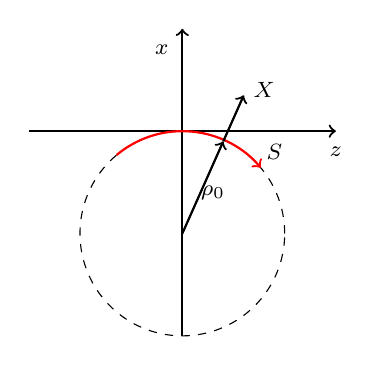
\begin{tikzpicture}[scale=1.3]
  \footnotesize
  % helper grid: comment for final drawing
  % \draw[help lines,step=.2] (0,0) grid (16.0,9.0);
  % \draw[help lines,line width=.6pt,step=1] (0,0) grid (16.0,9.0);
  % \foreach \x in {0,1,2,3,4,5,6,7,8,9,10,11,12,13,14,15,16}
  %      \node[anchor=north] at (\x,-0.1) {\x};
  % \foreach \y in {0,1,2,3,4,5,6,7,8,9}
  %     \node[anchor=east] at (-0.2,\y) {\y};

  % % text
  % \node [draw,rotate=90]  at (3.50,5.50)  {Injection};
  % % straight line and parabola
  % \draw [red,thick]          (0,0) -- (4,3);
  % \draw [black,thick,dashed] (0,0) parabola (4,4);
  % % bezier lines
  % \draw (6,0) .. controls (6,4) and (10,0) .. (10,4);
  % % circular shapes
  % \draw (5,5) circle (2cm);
  % \draw (7,2) ellipse (3cm and 1cm);
  % \draw (3,5) arc (0:75:3cm);
  % % filled rectangle



  % lower blms
%  \filldraw[fill=orange, draw=black] (9.2,3.8) rectangle (9.6,4.0);



  % % axes
  \draw[->,thick] (2,3) -- (5,3);
  \draw[->,thick] (3.5,1) -- (3.5,4);
  \draw[dashed] (3.5,2.0) circle (1.0);
  \draw[red,thick,->] (3.5,3.0) arc (90:40:1.0);
  \draw[red,thick,-] (3.5,3.0) arc (90:130:1.0);

  \draw[->,thick] (3.5,2) -- (3.9,2.9);
  \draw[->,thick] (3.9,2.9) -- (4.1,3.35);

  \node  at (3.8,2.4)  {$\rho_0$};
  \node  at (4.4,2.8)  {$S$};
  \node  at (5.0,2.8)  {$z$};
  \node  at (3.3,3.8)  {$x$};
  \node  at (4.3,3.4)  {$X$};

  % \draw[thick,->] (0,0) -- (0,4.5);

\end{tikzpicture}
  \caption{Transformation of the straight coordinate system $(x,y,z)$ into the curvilinear system $(X,Y,S)$. Based on \cite{wolski2014beam}.}
  \label{pic:16082101}
  \end{figure}







% %
%   \begin{figure}[b]
%   \centering
%   \includegraphics[width=0.25\textwidth]{pictures/15041701.png}
%   \caption{}  
%   \label{pic:15041701}
%   %/home/phermes/Desktop/curved.png
%   \end{figure}
%
In dipole magnets, the trajectory of the reference particle is curved. The motion of the particles in a dipole magnet is then most elegantly described in a curvilinear coordinate system. For the case of a purely horizontal and uniform bending magnet, the reference trajectory can be described by a bending radius $\rho_0$, as illustrated in Fig.~\ref{pic:16082101}. Based on the geometry, the coordinates in the straight ($x,y,z$) and in the curved coordinate system ($X,Y,S$) can be related to each other. With a third order generating function, the momentum coordinates in the curved coordinate system and the new magnetic potentials can be calculated. The derivation presented in the following is based on \cite{wolski2014beam}. From the geometry shown in Fig.~\ref{pic:16082101}, the new and old coordinates are related to each other by the simple equations:
\begin{align}
x &= (\rho_0 + X) \, \cos \left( \frac{S}{\rho_0} \right) - \rho_0 \, , \notag \\
y &= Y , \\
z &= (\rho_0 + X) \, \sin \left( \frac{S}{\rho_0} \right)  \notag \, .
\end{align}
One can construct a generating function of third order to calculate the particle momenta in the new coordinate system:
\begin{align}
F_3 (X,p_x,Y,p_y,S,p_z) = - \left[ (\rho_0 + X) \, \cos \left( \frac{S}{\rho_0} \right) - \rho_0 \right] \, p_x - Y \, p_y  - \left[ (\rho_0 + X) \, \sin \left( \frac{S}{\rho_0} \right) \right] \, p_z \, . \label{genF:rot}
\end{align}
%
The old and the new coordinates are then related by 
\begin{align}
x_i = - \PD{F_3}{p_i} \, \quad \quad P_i = - \PD{F_3}{X_i} \, .
\end{align}
The new momentum coordinates are given by
\begin{align}
P_X &= p_x \,  \cos \left( \frac{S}{\rho_0} \right) + p_z  \sin \left( \frac{S}{\rho_0} \right) \, , \notag \\
P_Y &= p_y \, , \\
P_S &= p_z \, \left( 1 + \frac{X}{\rho_0} \right)  \cos \left( \frac{S}{\rho_0} \right) - p_x \, \left( 1 + \frac{X}{\rho_0} \right)  \sin \left( \frac{S}{\rho_0} \right) \, . \notag
\end{align}
%
The vector potential is defined by
\begin{align}
A_X &= A_x \, \cos \left( \frac{S}{\rho_0} \right) - A_z \, \sin \left( \frac{S}{\rho_0} \right) \, , \notag \\
A_Y &= A_y \, , \\ 
A_S &= A_z \, \cos \left( \frac{S}{\rho_0} \right) + A_x \, \sin \left( \frac{S}{\rho_0} \right) \, , \notag 
\end{align}



\newpage

\section{Implementation of hiSixTrack} \label{chap:impl:hist}

The SixTrack source is saved altogether in the three files \lstinline{sixtrack.s}, \lstinline{lielib.s} and \mbox{\lstinline{dabnew.s}}. To build the SixTrack executable, a compilation file \lstinline{make_six} is executed with dedicated flags that activate given functionalities. Examples for such flags are the \lstinline{collimat} flag to compile the collimation version of SixTrack. An excellent overview of the compilation of SixTrack is given in \cite{Fjellstrom:1642385}. Specific functions of the SixTrack-FLUKA coupling are stored in an external module saved as \lstinline{mod_fluka.f90}. 



\subsection{Variables in hiSixTrack}

\begin{table}[b]
\centering
\caption{Variables in SixTrack~\cite{STdevwiki}. The variable \texttt{j} describes the particle index.}
\label{tab:sixtrack_variables}
\begin{tabular}{clccc}
\toprule
Variable             & Description                                   & Symbol     & Unit & Definition  \\ \midrule
%\texttt{j}           & particle index                                &                      &      &   \\
\texttt{napx}        & number of tracked particles                   &                      &      &   \\
\texttt{npart}       & maximum number of tracked particles           &                      &      &   \\ \midrule
 & \textbf{Reference particle properties} \\ \midrule
\texttt{e0}          & Energy of the reference particle              & $E_0$                & MeV  &                      \\
\texttt{e0f}         & Momentum of the reference particle            & $P_0$                & MeV/$c^2$  &                      \\ 
\texttt{pma}         & Proton rest mass            & $m_p$                & MeV/$c^2$  &               \\ \midrule
 & \textbf{Particle arrays} \\ \midrule
\texttt{xv(1,j)}     & Horizontal coordinate                         & $x$                  & mm   & \eqref{eq:refframe}  \\
\texttt{xv(2,j)}     & Vertical coordinate                           & $x$                  & mm   & \eqref{eq:refframe}  \\
\texttt{yv(1,j)}     & Horizontal slope                              & $x'$                 & mrad \\
\texttt{yv(2,j)}     & Vertical slope                                & $y'$                 & mrad \\
\texttt{sigmv(j)}    & Path length difference                        & $\sigma$             & mm   & \eqref{eq:sigmadefinition}  \\
\texttt{dpsv(j)}     & Relative momentum offset                      & $\delta$             & -    &  \eqref{delta:mono}    \\
\texttt{oidpsv(j)}   & Relative momentum offset                      & $\frac{1}{1+\delta}$ & -    &     \\
\texttt{ejfv(j)}     & Particle momentum                             & $P$                  & MeV/$c$    &     \\
\texttt{ejv(j)}      & Particle energy                               & $E$                  & MeV    &     \\ \bottomrule
\end{tabular}
\end{table}




\begin{table}[b]
\centering
\caption{Variables introduced or modified in hiSixTrack. The variable \texttt{j} describes the particle index.}
\label{tab:hisixtrack_variables}
\begin{tabular}{clccc}
\toprule
Variable             & Description           & Symbol & Unit & Definition\\ \midrule
 & \textbf{Reference particle properties} \\ \midrule
\texttt{zz0}           &  Charge multiplicity of the reference ion species    & $Z_0$     & - &       \\
\texttt{aa0}           &  Nucleon number of the reference ion species         & $A_0$     & - &       \\
\texttt{nucm0}         &  Rest mass of the reference ion species              & $m_0$     & GeV/$c^2$ &       \\ \midrule
 & \textbf{Particle arrays} \\ \midrule
\texttt{nzz(j)}        &  Charge multiplicity of the tracked ion              & $Z$       & - &       \\
\texttt{naa(j)}        &  Nucleon number of the tracked ion                   & $A$       & - &       \\
\texttt{nucm(j)}       &  Rest mass of the tracked ion                        & $m$       & GeV/$c^2$ & \\
\texttt{mtc(j)}        &  Relative mass to charge ratio                       & $\chi$    & - & \eqref{eq:chidef}      \\
\texttt{dpsv(j)}       &  Relative \textbf{momentum per mass} offset          & $\delta$  & -    & \eqref{eq:15010701}     \\
\texttt{moidpsv(j)}    &  Relative rigidity offset  & $\frac{\chi}{1+\delta}$    & - &   \eqref{eq:brho_brho0}   \\ \bottomrule
\end{tabular}
\end{table}

SixTrack tracks a variety of different arrays, to store information of the tracked particle bunch. Besides the obvious arrays \lstinline{xv(i,j),yv(i,j),sigmv(j),dpsv(j)} containing information about the six-dimensional particle coordinates, other arrays store information about the particle energy and momentum as well as auxiliary quantities derived from them. In the process of tracking, the latter are re-initialized every time the particle momentum (and in hiSixTrack the particle species) may have changed, which is true for the collimators and accelerating elements. An overview of the most relevant particle arrays is given in \tabref{tab:sixtrack_variables}.

Some of these variables are redefined in hiSixTrack in order to be compatible with the generic multi-isotopic definitions introduced in \chapref{transverse:ions}. This includes the relative offset of the momentum per mass unit $\delta$ which is implemented in the SixTrack as the relative momentum offset. Furthermore, new variables are introduced to keep track of the particle species and to facilitate the implementation of the heavy-ion tracking maps. These variables are summarized in \tabref{tab:hisixtrack_variables}. For the identification of the tracked particles, the mass number $A$, the charge multiplicity $Z$ and rest mass $m$ are stored in arrays. The latter is not important for the identification of the particle, but it is used to calculate $\chi$. The information about the reference species $A_0,Z_0,m_0$ is read from \lstinline{fort.3} with a newly introduced block \lstinline{HION}, described in the next subsection. 

The implementation of $\delta$ in both SixTrack and hiSixTrack is shown in \lstref{lst_delta}. The quantity $ \frac{\delta}{1+\delta}$ follows the redefinition of $\delta$.

\vspace{0.5cm}
\begin{minipage}{\linewidth}
\begin{lstlisting}[language=Fortran,caption=Definition of $\delta$ in SixTrack and hiSixTrack.,label=lst_delta]
!        dpsv  (j)   = (ejfv(j)-e0f)/e0f                    ! SixTrack
         dpsv  (j)   = (ejfv(j)*(nucm0/nucm(j))-e0f)/e0f    ! hiSixTrack
         oidpsv(j)   = one/(one+dpsv(j))
\end{lstlisting}
\end{minipage}


The quantity \lstinline{mtc(j)} represents the relative mass to charge ratio $\chi$. Its definition in the SixTrack source is shown in \lstref{lst_chi}. 

\vspace{0.5cm}
\begin{minipage}{\linewidth}
\begin{lstlisting}[language=Fortran,caption=Definition of $\chi$ in hiSixTrack.,label=lst_chi]
        mtc     (j) = (nzz(j)*nucm0)/(zz0*nucm(j)) 
\end{lstlisting}
\end{minipage}

Note that instead of using the particle charge $q$, hiSixTrack uses the nuclear charge multiplicity $Z$, assuming that all electrons are removed from the tracked particle and the reference particle. If non-fully stripped ions should be tracked with hiSixTrack, the source has to be extended for an additional array storing the effective ion charge. The variable \lstinline{moipdsv(j)} describes the auxiliary quantity $\frac{\chi}{1+\delta}$ representing the relative offset in magnetic rigidity.

While in SixTrack the particle mass is hard coded as a constant parameter \lstinline{pma} that is applied for all particles, hiSixTrack requires a new implementation of mass-dependent equations in which the particle mass is a variable. Depending on the context, \lstinline{pma} refers to the mass of the reference particle or of the tracked particle and is replaced in hiSixTrack by \lstinline{nucm0} or \lstinline{nucm(j)} accordingly. In  \lstref{listing_einstein}, the Einstein energy-momentum relation is shown as it is implemented in SixTrack and hiSixTrack for both the reference particle and for a tracked particle.
\vspace{0.5cm}

\begin{minipage}{\linewidth}
\begin{lstlisting}[language=Fortran,caption=Definition of the reference momentum $P_0$ and the energy $E$ of the tracked ion in SixTrack and hiSixTrack.,label=listing_einstein]
!        MOMENTUM OF THE REFERENCE PARTICLE
!        e0f=sqrt(e0**2-pma**2)              ! SixTrack
         e0f=sqrt(e0**2-nucm0**2)            ! hiSixTrack
!
!        ENERGY OF THE TRACKED ION j
!        ejv(j)=sqrt(ejfv(j)**2+pma**2)      ! SixTrack
         ejv(j)=sqrt(ejfv(j)**2+nucm(j)**2)  ! hiSixTrack
\end{lstlisting}
\end{minipage}

\subsection{Initialization of hiSixTrack}

hiSixTrack is activated by calling the new \lstinline{HION} block in the fort.3 file. This block acquires information on the reference particle species ($A_0,Z_0,m_0$). The code defining the HION block in the hiSixTrack source code is shown in \lstref{lst:hion_src}. An example input block to call hiSixTrack for different heavy-ion reference species is given in \lstref{lst:f3hi}.


\vspace{0.5cm}
\begin{minipage}{\linewidth}
\begin{lstlisting}[language=Fortran,caption=Definition of the information acquisition from the \lstinline{fort.3} in the hiSixTrack source file.,label=lst:hion_src]
!     P. HERMES 01-07-2015
!     HEAVY ION BLOCK
 2400 read(3,10020,end=1530,iostat=ierro) ch
      if(ierro.gt.0) call prror(58)
      if(ch(1:1).eq.'/') goto 2400
      if(ch(:4).eq.next) goto 110
      ch1(:nchars+3)=ch(:nchars)//' / '
      read(ch1,*) aa0, zz0, nucm0
      nucm0 = nucm0  * 1.0D+03 !  [GeV/c^2] -> [MeV/c^2] ! hiSixTrack
      write(*,*) 'Heavy-ion reference species:', aa0, zz0, nucm0
      goto 110
\end{lstlisting}
\end{minipage}


\vspace{0.5cm}
\begin{minipage}{\linewidth}
\begin{lstlisting}[language=Fortran,caption={New heavy-ion block in the fort.3 file to activate hiSixTrack. In the given example, the chosen reference ion species is \lead. Lines starting with '/' are commented out.}, label={lst:f3hi}]
HION
/1     1    0.9382723             /PROTONS
/40   18    37.215549             /ARGON IONS
/129  54    120.04664             /XENON IONS
208   82    193.68769             /LEAD IONS
NEXT
\end{lstlisting}
\end{minipage}

\subsection{Initial Particle Distribution}

In the framework of the SixTrack-FLUKA coupling, SixTrack provides subroutine \lstinline{dist_readdis} to load an initial distribution from an external file. The subroutine is called by the \lstinline{DIST} block in the fort.3 file. For hiSixTrack, the routine is adapted to read also $A,Z$ and the particle mass $m$. Already the implementation in SixTrack foresaw different isotopes, so only minor changes are required to access the heavy-ion specific properties from the input file.

When the initial distribution is sampled from the input file, the acquired quantities are processed to populate the respective arrays for the tracking. The modification includes the new definition of $\delta$, the correct nuclear rest mass (as shown in the previous subsection), the initialization of $\chi$ and auxiliary quantities derived from it. The relevant code is shown in \lstref{lst_dist_readdis}.


\vspace{0.5cm}
\begin{minipage}{\linewidth}
\begin{lstlisting}[language=Fortran,caption=Definition of the subroutine \lstinline{dist_readdis} in hiSixTrack including the initialization of $\chi$ and auxiliary quantities as well as the redefined $\delta$.,label=lst_dist_readdis]
         call dist_readdis( napx, npart, enom, pnom, clight,
     &                         x, y, xp, yp, s, pc, aa, zz, m )
!        [...]         
!        LOOP OVER ALL PARTICLES
         do j=1, napx
!            VALUES RELATED TO LOSSES
             nlostp(j) = j
             pstop (j) = .false.
!            VALUES RELATED TO MOMENTUM (MODIFIED IN HISIXTRACK)
             ejv   (j)   = sqrt(ejfv(j)**2+nucm(j)**2)	             
             dpsv  (j)   = (ejfv(j)*(nucm0/nucm(j))-e0f)/e0f
             oidpsv(j)   = one/(one+dpsv(j))
!            NEW IN HISIXTRACK
             mtc     (j) = (nzz(j)*nucm0)/(zz0*nucm(j))  
             moidpsv (j) = mtc(j)*oidpsv(j)
             omoidpsv(j) = c1e3*((one-mtc(j))*oidpsv(j))
!       [...]
\end{lstlisting}
\end{minipage}




\subsection{Implemented Heavy-Ion Tracking Maps} \label{chap:implement}

Some of the redefined tracking maps in hiSixTrack are shown in \lstref{lst:kickermagnet} to \lstref{lst:quadkick}. 


\vspace{0.5cm}
\begin{minipage}{\linewidth}
\begin{lstlisting}[language=Fortran,caption=Definition of the transfer map of an horizontal kicker dipole.,label=lst:kickermagnet]
+cd kickv01h
+if .not.tilt
!            yv(1,j)=yv(1,j)+(strack(i)*oidpsv(j))        ! SixTrack
            yv(1,j)=yv(1,j)+(strack(i)*oidpsv(j))*mtc(j)  ! hiSixTrack
+ei
+if tilt
            yv(1,j)=yv(1,j)+(strackc(i)*oidpsv(j))*mtc(j) 
            yv(2,j)=yv(2,j)+(stracks(i)*oidpsv(j))*mtc(j) 
+ei
\end{lstlisting}
\end{minipage}

\vspace{0.5cm}
\begin{minipage}{\linewidth}
\begin{lstlisting}[language=Fortran,caption=Definition of the transfer map of a vertical dipole kick.]
+cd kickv01v
+if .not.tilt
            yv(2,j)=yv(2,j)+(strack(i)*oidpsv(j))*mtc(j)  ! hiSixTrack
+ei
+if tilt
            yv(1,j)=yv(1,j)-(stracks(i)*oidpsv(j))*mtc(j) ! hiSixTrack
            yv(2,j)=yv(2,j)+(strackc(i)*oidpsv(j))*mtc(j) ! hiSixTrack
+ei
\end{lstlisting}
\end{minipage}

\vspace{0.5cm}
\begin{minipage}{\linewidth}
\begin{lstlisting}[language=Fortran,caption=Definition of the transfer map of a quadrupole.,label=lst:quadkick]
+cd kickvxxh
+if .not.tilt
            yv(1,j)=yv(1,j)+((strack(i)*oidpsv(j))*crkve)*mtc(j) ! hiSixTrack
            yv(2,j)=yv(2,j)-((strack(i)*oidpsv(j))*cikve)*mtc(j) ! hiSixTrack
+ei
+if tilt
            yv(1,j)=yv(1,j)+(oidpsv(j)*(strackc(i)*crkve+               &
     &stracks(i)*cikve))*mtc(j)
            yv(2,j)=yv(2,j)+(oidpsv(j)*(stracks(i)*crkve-               &!hr02
     &strackc(i)*cikve))*mtc(j)                                          !hr02
+ei
\end{lstlisting}
\end{minipage}



% \vspace{0.5cm}
% \begin{minipage}{\linewidth}
% \begin{lstlisting}[language=Fortran,caption=Definition of the transfer map of a vertical dipole kick.,label=lastmap]
% +cd kickvxxv
% +if .not.tilt
%             yv(1,j)=yv(1,j)+((strack(i)*oidpsv(j))*cikve)*mtc(j) ! hiSixTrack
%             yv(2,j)=yv(2,j)+((strack(i)*oidpsv(j))*crkve)*mtc(j) ! hiSixTrack
% +ei
% +if tilt
%             yv(1,j)=yv(1,j)+(oidpsv(j)*(strackc(i)*cikve-               &
%      &stracks(i)*crkve))*mtc(j)
%             yv(2,j)=yv(2,j)+(oidpsv(j)*(strackc(i)*crkve+               &
%      &stracks(i)*cikve))*mtc(j)
% +ei
% \end{lstlisting}
% \end{minipage}

\section{Implementation of the hiSixTrack-FLUKA Coupling} \label{coupling:imp}

\subsection{Code Structure}

The SixTrack-FLUKA coupling requires several changes with respect to the standalone tools to provide particle exchange between the different codes. The most important ingredient is the FlukaIO protocol, developed for this purpose~\cite{flukaiotwiki}. Before the set up of hiSixTrack, this protocol was already equipped with a function to send information about $A,Z,m$ back and forth. Only minor modifications (implemented by V. Vlachoudis) were necessary to adapt the FlukaIO for the hiSixTrack-FLUKA coupling. 

Both the FLUKA input and subroutines, as well as the SixTrack source are adapted to allow for the exchange of information about the heavy-ion species. These changes are summarized below.


\subsection{Changes in FLUKA Input and Subroutines}

This subsection gives a brief overview of the modifications at the FLUKA user routines, input file and compilation to allow for the accurate heavy-ion exchange and an appropriate fragmentation simulation. 

\subsubsection{Initialization and Particle Reception}

The communication between FLUKA and the FlukaIO is established via the user routine \texttt{source.f}~\cite{couplingtwiki}. The human interface to control the latter is the \texttt{SOURCE} card in the FLUKA input file. It is used to receive the particle distribution from SixTrack and write the \texttt{toucMap} file.  For the coupling with hiSixTrack, the \texttt{source.f} user routine is modified to ensure the accurate initialization of the FLUKA particle variables (author: A. Mereghetti). The function to write the \texttt{toucMap} file is extended for heavy-ion applications by saving additional information on $A,Z$.

\subsubsection{Sending Particles back to hiSixTrack} \label{chap:correctionfile}

The particle bunch is sent back to hiSixTrack via the user routine \texttt{fluscw.f}, which is activated over the \texttt{USRBDX} card with the special \texttt{SDUM} keyword \texttt{BACK2ICO} (see \cite{couplingtwiki}). In this user routine the particles are selected and the \texttt{fort.66} file containing the correction data for the collimator losses is populated as shown in \lstref{lst:fluscw}. The user routine is activated when the boundary crossing condition is fulfilled (in this framework a transition from the vacuum surrounding the collimators to black absorber). The type of boundary crossing is defined in the \texttt{USRBDX} card, as shown in \lstref{lst:usrbdx}, for the nominal SixTrack-FLUKA coupling on top and for the heavy-ion version on the bottom. 

\vspace{0.5cm}
\begin{minipage}{\linewidth}
\begin{lstlisting}[language=Fortran,caption=Particle selection in the \texttt{fluscw.f} user routine to write the data to the collimator loss correction file \texttt{fort.66}.,label=lst:fluscw]
     [...]
            ESCO = -PLA + AM(IJ)
*           hiST: write all particles not sent back to fort.66
            IF ( IJ .GT. 0 .OR. IJ .LT. -6 ) THEN
                WRITE(66,*) 
     &                 IJ, IBARCH(IJ), ICHRGE(IJ),ICPPNT,ESCO
            RETURN
            END IF
    [...]
\end{lstlisting}
\end{minipage}

\vspace{0.5cm}
\begin{minipage}{\linewidth}
\begin{lstlisting}[language=Fortran,caption=USRBDX card in the FLUKA input for the nominal SixTrack-FLUKA coupling (commented out) and the heavy-ion version at the bottom.,label=lst:usrbdx]
*USRBDX          99.0    PROTON     -42.0   VAROUND  BLKROUND          BACK2ICO
*USRBDX        8000.0   1.0E-04     210.0                              &
USRBDX          99.0  ALL-PART     -42.0   VAROUND  BLKROUND          BACK2ICO
USRBDX      576000.0   1.0E-04     210.0                   
\end{lstlisting}
\end{minipage}


\subsubsection{Compilation}

The computation of high-energy hadronic interactions in FLUKA requires the activation of the DPMJET-III~\cite{MC2000:DPMJETIII}. For this purpose, the linking of the user routines is done with a different linker, which is incorporated in the FLUKA \texttt{Makefile} in the framework of the hiSixTrack-FLUKA coupling where the usage of the default \texttt{lfluka} linker is replaced by \texttt{ldpm3qmd}.



\subsubsection{Input File}

Besides the changes on the \texttt{USRBDX} card mentioned above, minor changes at the FLUKA input make the framework compatible for heavy-ion applications. The \texttt{SDUM} of the \texttt{BEAM} card is changed from \texttt{PROTON} to \texttt{HEAVYION} with the subsequent definition of the main beam isotope. Furthermore, heavy-ion specific EMD and nuclear evaporation are activated by means of their dedicated cards, as shown in \lstref{lst:input}.

\vspace{0.5cm}
\begin{minipage}{\linewidth}
\begin{lstlisting}[language=Fortran,caption=Changes in the FLUKA input for heavy-ion applications,label=lst:input]
* activate EMD and Evaporation for heavy-ions 
PHYSICS          2.0                                                  EM-DISSO 
PHYSICS     3.0                                                       EVAPORAT
* maximum momentum per nucleon (3000 for 3.5Z TeV, 6000 for 6.37Z TeV)
BEAM           6000.                                                  HEAVYION
HI-PROPE         82.      208.                                                
*
\end{lstlisting}
\end{minipage}


\subsection{Changes in hiSixTrack} \label{app:changeshist}
Several modifications are required in hiSixTrack to adapt the software for the exchange of heavy-ions. The most important changes are done in the subroutine \texttt{kernel\_fluka\_entrance} and the \texttt{kernel\_fluka\_exit}.

\vspace{0.5cm}
\begin{minipage}{\linewidth}
\begin{lstlisting}[language=Fortran,caption=Send particles to FLUKA as implemented in hiSixTrack.,label=lst:coupling_send]
      subroutine kernel_fluka_entrance( nturn, i, ix )
      use mod_fluka
      [...]
+ca hions                            ! load the commons specific to hiST
      [...]	
      nnuc0 = 0                      ! nucleons sent to FLUKA
      ien0  = 0.0                    ! ion energy sent to FLUKA

      do j=1,npart                   ! initialize array of particle ids 
         pids(j) = 0
      end do
	
      do j=1,napx                    
         nnuc0   = nnuc0 + naa(j)    ! count nucleons
         ien0    = ien0  + ejv(j)    ! count energy [GeV]
         pids(j) = fluka_uid(j)      ! array of SixTrack IDs sent to FLUKA
      end do

      ret = fluka_send( nturn, fluka_geo_index(ix), eltot, napx,        &
     & xv(1,:), yv(1,:), xv(2,:), yv(2,:), sigmv, ejv , naa(:), nzz(:), &
     &nucm(:) ) 

     [...]
     return
     end subroutine
\end{lstlisting}
\end{minipage}

\paragraph{kernel\_fluka\_entrance}
This subroutine sends the particle bunch to FLUKA via the dedicated function \texttt{fluka\_send}. For hiSixTrack, the number of nucleons (\texttt{nnuc0}) and the total particle energy (\texttt{ien0}) sent to FLUKA are counted before the particle bunch is sent to FLUKA. This information is compared to the total nucleon number and particle energy when the bunch of residual ions is sent back from FLUKA to SixTrack, to calculate the ion loss (see paragraph below). Furthermore a dedicated array (\texttt{pids(j)}) containing the hiSixTrack particle IDs of all particles sent to FLUKA is populated, to save the particle information about the particles lost at the collimator.  The most important changes are shown in \lstref{lst:coupling_send}.


\paragraph{kernel\_fluka\_exit}
\mbox{} \\
The subroutine \texttt{kernel\_fluka\_exit} is called when the particle bunch is sent back from FLUKA to hiSixTrack. It makes use of the \texttt{fluka\_receive} subroutine defined in the \texttt{mod\_fluka} module. After the bunch of residual particles is received by the \texttt{fluka\_receive} function, the arrays storing the particle momenta, $\delta$, $\chi$ and other quantities are re-populated. Also, the number of out-scattered nucleons (\texttt{nnuc1}) and the integrated energy of the received particle bunch (\texttt{ien1}) are calculated. In a subsequent step, the latter are compared to \texttt{nnuc0} and \texttt{ien0} to calculate the collimator losses, which are saved into the \texttt{fort.208} file. In a last step, it is identified which particle IDs have been sent to FLUKA but not back to SixTrack. The corresponding particle information is then saved in to the \texttt{fort.209} file. The implementation in hiSixTrack is shown in \lstref{lst:coupling_rec}.

\vspace{0.5cm}
\begin{minipage}{\linewidth}
\begin{lstlisting}[language=Fortran,caption=Receive particles from FLUKA as implemented in hiSixTrack.,label=lst:coupling_rec]

      subroutine kernel_fluka_exit( nturn, i, ix )
      [...]
      ret = fluka_receive( nturn, fluka_geo_index(ix), eltot, napx,     &
     &xv(1,:), yv(1,:), xv(2,:), yv(2,:), sigmv, ejv, naa(:),nzz(:)     &
     & ,nucm(:) ) 
      nnuc1 = 0                 ! init. number of nucleons leaving collimator
      ien1  = 0.0               ! init. total energy leaving collimator
      do j=1,napx
         [...]
!        Update hiST arrays (naa, nzz, nucm are initialized by fluka_receive)
         ejfv    (j) = sqrt((ejv(j)-nucm(j))*(ejv(j)+nucm(j))) ! ion momentum
         rvv     (j) = (ejv(j)*e0f)/(e0*ejfv(j))               ! beta0/beta
         dpsv    (j) = (ejfv(j)*(nucm0/nucm(j))-e0f)/e0f       ! delta
         oidpsv  (j) = 1.0D+00/(1.0D+00+dpsv(j))               ! 1/(1+delta)
         dpsv1   (j) = (dpsv(j)*1.0D+03)*oidpsv(j)             ! 
         mtc     (j) = (nzz(j)*nucm0)/(zz0*nucm(j))            ! chi
         moidpsv (j) = mtc(j)*oidpsv(j)                        ! chi/(1+delta)
         omoidpsv(j) = 1.0D+03*((1.0D+00-mtc(j))*oidpsv(j))    ! 
         nnuc1       = nnuc1 + naa(j)                          ! increase nucleon counter
         ien1        = ien1  + ejv(j)                          ! increase energy counter
      end do
      ! hiSixTrack: if energy is lost at the collimator, write to fort.208
        if ((ien0-ien1).gt.one) then
            write(208,*), fluka_geo_index(ix), nnuc0-nnuc1,             &
     &     (ien0-ien1)*1d-3
        end if
!     hisix: check which particle ids have not been sent back
!            write their ids to fort.209
      do j=1,npart                                       ! loop over all IDs
	  pid_q = zero
	  do k=1,napx                                    ! loop over pids received
	      if (pids(j).eq.fluka_uid(k)) then
	          pid_q = one
	      end if
	  end do
	  if (pid_q.eq.zero.and.pids(j).ne.zero) then
              write(209,*), fluka_geo_index(ix), pids(j)
	  end if
      end do
\end{lstlisting}
\end{minipage}



\end{appendices}



\chapter*{Publications}

This is a summary of publications the author published during the work on the Ph.D. project.
\\ \mbox{} \\ 
\large{\textbf{Main Author}}
\normalsize
%
\\ \mbox{} \\
\textit{Journal Paper}
%
\\ \mbox{} \\
P.~D. Hermes, R. Bruce, J.~M. Jowett, S. Redaelli, B. Salvachua, G. Valentino, \mbox{D. Wollmann},  \\
``\textit{Measured and Simulated Heavy-Ion Beam Loss Patterns at the CERN Large Hadron Collider}'' \newline 
Nuclear Instruments and Methods in Physics Research A 819 (2016) 73-83.
%
\\ \mbox{} \\
\textit{Proceedings}
\\ \mbox{} \\
P.~D.~Hermes, R. Bruce, F. Cerutti, A. Ferrari, J.~M. Jowett, A. Lechner, A. Mereghetti, \mbox{D. Mirarchi}, P.~G. Ortega, S. Redaelli, B. Salvachua, E. Skordis, G. Valentino, V. Vlachoudis, \\ 
``\textit{Simulation of Heavy-Ion Beam Losses with the SixTrack-FLUKA Active Coupling}'' \newline
Proceedings of IPAC 2016 (WEPMW029):2490-2493, Busan, Korea. 
%
\\ \mbox{} \\
P.~D.~Hermes, R. Bruce, R. De Maria, \\ 
``\textit{Symplectic Tracking of Multi-Isotopic Heavy-Ion Beams in SixTrack}'' \newline
Proceedings of IPAC 2016 (TUPMW015):1450-1453, Busan, Korea. 
%
\\ \mbox{} \\
P.~D. Hermes, R. Bruce, M. Fiascaris, H. Garcia, M. Giovannozzi, A. Mereghetti, D. Mirarchi, E. Quaranta, S. Redaelli, B. Salvachua, G. Valentino, R. Kwee-Hinzmann, E. Quaranta \\ 
``\textit{Improved Aperture Measurements at the LHC and Results from their Application in 2015}'' \newline
Proceedings of IPAC 2016 (TUPMW014):1446-1449, Busan, Korea. 
% 	
%\\ \mbox{} \\
\newpage
P.~D.~Hermes, R.~Bruce, J.~M.~Jowett, S.~Redaelli, \\ 
``\textit{Betatron Cleaning for Heavy Ion Beams with IR7 Dispersion Suppressor Collimators}'' \newline
Proceedings of IPAC 2015 (TUPTY025):2057-2059, Richmond, VA, USA. 
%
\\ \mbox{} \\
P.~D. Hermes, R. Bruce, J.M. Jowett, S. Redaelli, B. Salvachua, G. Valentino, D. Wollmann,  \\ 
``\textit{Studies on Heavy Ion Losses from Collimation Cleaning at the LHC}'' \newline
Proceedings of HB 2014 (MOPAB43):138-142, East Lansing, MI, USA. 
\\ \mbox{} \\
\textit{CERN Publications}
\\ \mbox{} \\
%
P.~D. Hermes, B. Auchmann, R. Bruce, W. H\"{o}fle, E.~B. Holzer, M. Kalliokoski, G. Kotzian, A. Mereghetti, D. Mirarchi, E. Quaranta, S. Redaelli, G. Valentino, D. Valuch, D. Wollmann, \mbox{M. Zerlauth}, ``\textit{LHC Heavy-Ion Collimation Quench Test at 6.37$\,Z\,$TeV}'' \newline
CERN-ACC-NOTE-2016-0031, CERN, Geneva, Switzerland, (2016).
%
\\ \mbox{} \\
\large{\textbf{Co-Author}}
\normalsize
%
\\ \mbox{} \\
\textit{Proceedings}
%
% \cvitem{2016}{\textbf{\textit{Performance of the LHC collimation system during 2015}} \newline
% G. Valentino, R. Bruce, M. Fiascaris, H. Garcia, P. D. Hermes \textit{et al.},\newline
% % , A. Mereghetti, D. Mirarchi, R. Kwee, S. Redaelli, E. Quaranta, A. Rossi, R. Rossi, B. Salvachua, P. Theodoropoulos, A. Valloni, J. Wagner
% \textit{Proceedings of the 6th Evian Workshop}, Evian, France (2015)}
%
%
\\ \mbox{} \\
J.M. Jowett, R. Alemany-Fernandez, R. Bruce, M. Giovannozzi, P.~D. Hermes, W. H\"{o}fle, \mbox{M. Lamont}, T. Mertens, S. Redaelli, M. Schaumann, J.A. Uythoven, J. Wenninger, \\ 
``\textit{The 2015 Heavy-Ion Run of the LHC}'' \newline
Proceedings of IPAC 2016 (TUPMW027):1493-1496, Busan, Korea. 
% 	
\\ \mbox{} \\
B. Salvachua, P. Baudrenghien, R. Bruce, H. Garcia, P.~D. Hermes, S. Jackson, M. Jaussi, \mbox{A. Mereghetti}, D. Mirarchi, S. Redaelli, H. Timko, G. Valentino, A. Valloni, R. Kwee-Hinzmann, \\ 
``\textit{Validation of Off-momentum Cleaning Performance of the LHC Collimation System}'' \newline
Proceedings of IPAC 2016 (WEPMW007):2427-2430, Busan, Korea. 
% 	 	
\\ \mbox{} \\
D. Mirarchi, A. Bertarelli, R. Bruce, F. Cerutti, P.D. Hermes, A. Lechner, A. Mereghetti, \mbox{E. Quaranta}, S. Redaelli, R.B. Appleby, H. Garcia Morales, R. Kwee-Hinzmann, \\ 
``\textit{Cleaning Performance of the Collimation System of the High Luminosity Large Hadron Collider}'', Proceedings of IPAC 2016 (WEPMW030):2494-2497, Busan, Korea. 
% 	 	
%\\ \mbox{} \\
\newpage
E. Quaranta, A. Bertarelli, F. Carra, P.~D. Hermes, S. Redaelli, A. Rossi, K. Bunk, F. Carra, J. Guardia Valenzuela, C.L. Hubert, M. Tomut, P. Nocera, C. Porth, N. Simos, \\ 
``\textit{Radiation-induced Effects on LHC Collimator Materials under Extreme Beam Conditions}'' \newline
Proceedings of IPAC 2016 (WEPMW032):2502-2505, Busan, Korea. 
%
\\ \mbox{} \\
%D. Mirarchi, R. Bruce, M. Giovannozzi, P. D. Hermes, S. Redaelli, ``\textit{LHC aperture and ULO restrictions: are they a possible limitation in 2016?}'' \newline
%Proceedings of the 6th Evian Workshop,  Evian, France, (2015).
%\\ \mbox{} \\
D. Mirarchi, R. Bruce, M. Giovannozzi, P. D. Hermes, S. Redaelli, B. Salvachua, G. Valentino, J. Wenninger,  
``\textit{LHC aperture and ULO restrictions: are they a possible limitation in 2016?}'' \newline
Proceedings of the 6th Evian Workshop,  Evian, France, (2015).
\\ \mbox{} \\
G. Valentino, R. Bruce, M. Fiascaris, H. Garcia, P. D. Hermes, A. Mereghetti, \mbox{D. Mirarchi}, \mbox{R. Kwee}, S. Redaelli, E. Quaranta, A. Rossi, R. Rossi, B. Salvachua, P. Theodoropoulos, \mbox{A. Valloni}, J. Wagner, ``\textit{Performance of the LHC collimation system during 2015}'' \newline
Proceedings of the 6th Evian Workshop, Evian, France (2015).
\\ \mbox{} \\ 	 	
% 	 	
E. Skordis, R. Bruce, F. Cerutti, A. Ferrari, P.D. Hermes, A. Lechner, A. Mereghetti, \mbox{P.G. Ortega}, S. Redaelli, V. Vlachoudis, \\ ``\textit{Impact of Beam Losses in the LHC Collimation Regions}'' \newline
Proceedings of IPAC 2015 (TUPTY046):2116-2119, Richmond, VA, USA. 
%
\\ \mbox{} \\
\textit{CERN Publications}
\\ \mbox{} \\
B. Salvachua, A. Mereghetti, B. Auchmann, R. Bruce, P.D. Hermes, E.B. Holzer, D. Jacquet, M. Kalliokoski, D. Mirarchi, S. Redaelli, E. Skordis, G. Valentino, A. Valloni, D. Valuch, \mbox{D. Wollmann}, M. Zerlauth,  
``\textit{Collimation Quench Test with 6.5 TeV Proton Beams}'' \newline
CERN-ACC-NOTE-2016-0015, CERN, Geneva, Switzerland (2016).
\\ \mbox{} \\
R. Bruce, P. D. Hermes, H. Garcia, R. Kwee-Hinzmann, A. Mereghetti, D. Mirarchi, S. Redaelli, B. Salvachua, P. Skowronski, G. Valentino, A. Valloni,  \\
``\textit{IR aperture measurement at $\beta^* =$40 cm}'' \newline
CERN-ACC-NOTE-2015-0037, CERN, Geneva, Switzerland (2015).
\\ \mbox{} \\
R. Bruce, H. Garcia, P.D. Hermes, R. Kwee-Hinzmann, A. Mereghetti, D. Mirarchi, \mbox{E. Quaranta}, S. Redaelli, B. Salvachua, G. Valentino, A. Valloni, \\ 
``\textit{Collimation with tighter TCTs at $\beta^*=$40 cm}'' \newline
CERN-ACC-NOTE-2015-0036, CERN, Geneva, Switzerland (2015).
%\\ \mbox{} \\
\newpage
G. Valentino, G. Baud, R. Bruce, H. Garcia, P. D. Hermes, M. Gasior, R. Kwee, D. Mirarchi, J. Olexa, S. Redaelli, R. Rossi, B. Salvachua, A. Valloni, J. Wagner, \\
``\textit{Characterization of Embedded BPM Collimators}'' \newline
CERN-ACC-NOTE-2015-0027, CERN, Geneva, Switzerland (2015).






% \cvitem{2016}{\textbf{\textit{Collimation quench test with 6.5 TeV proton beams}} \newline 
% B. M. Salvachua Ferrando, B. Auchmann, R. Bruce, P. D. Hermes, E. Holzer \textit{et al.}, 
% % D. Jacquet, M. Kalliokoski, A. Mereghetti, D. Mirarchi, S. Redaelli, E. Skordis, G. Valentino, A. Valloni, D. Wollmann, M. Zerlauth 
% \textit{CERN-ACC-NOTE-2016-0015}, CERN, Geneva, Switzerland}

% \cvitem{2015}{\textbf{\textit{IR aperture measurement at $\beta^*=$40 cm}} \newline 
% \mbox{R. Bruce, H. Garcia Morales, P. D. Hermes, R. Kwee-Hinzmann, A. Mereghetti \mbox{\textit{et al.}}},
% % , D. Mirarchi, S. Redaelli, B. M. Salvachua Ferrando, P. K. Skowronski, G. Valentino, A. Valloni,
% \textit{CERN-ACC-NOTE-2015-0037}, CERN, Geneva, Switzerland}

% \cvitem{2015}{\textbf{\textit{Collimation with tighter TCTs at $\beta^*=$40 cm}} \newline 
% \mbox{R. Bruce, H. Garcia Morales, P. D. Hermes, R. Kwee-Hinzmann, A. Mereghetti \mbox{\textit{et al.}}},
% % , D. Mirarchi, E. Quaranta, S. Redaelli, B. M. Salvachua Ferrando, G. Valentino, A. Valloni,
% \mbox{\textit{CERN-ACC-NOTE-2015-0036}}, CERN, Geneva, Switzerland}

% \cvitem{2015}{\textbf{\textit{Characterization of Embedded BPM Collimators}} \newline G. Valentino, G. Baud, R. Bruce, H. Garcia, P. D. Hermes \mbox{\textit{et al.}},
% % , M. Gasior, R. Kwee, D. Mirarchi, J. Olexa, S. Redaelli, R. Rossi, B. Salvachua, A. Valloni, J. Wagner, 
% \mbox{\textit{CERN-ACC-NOTE-2015-0028}}, CERN, Geneva, Switzerland}

% \cvitem{2015}{\textbf{\textit{Impact of Beam Losses in the LHC Collimation Regions}} \newline 
% \mbox{E.~Skordis, R.~Bruce, F.~Cerutti, A.~Ferrari, P.~D.~Hermes \textit{et al.}}
% %, A.~Lechner, A.~Mereghetti, P.~G.~Ortega, S.~Redaelli, V.~Vlachoudis, 
% \newline
% \textit{Proc. of IPAC 2015 (TUPTY046)}, Richmond, VA, USA}


% \cvitem{2013}{\textbf{\textit{IR2 Aperture Measurements at 4.0 TeV}} \newline R.~Bruce, M.~Giovannozzi, P.~D.~Hermes, S.~Redaelli, J.~Wenninger, \mbox{\textit{CERN-ACC-NOTE-2013-0011}}, CERN, Geneva, Switzerland} 

% \cvitem{2013}{\textbf{\textit{IR8 Aperture Measurements at injection energy}} \newline R.~Bruce, M.~Giovannozzi, P.~D.~Hermes, B.~Holzer, A.~A.~Nosych \textit{et al.}, 
% \mbox{\textit{CERN-ATS-Note-2013-026 MD}}, CERN, Geneva, Switzerland} 
\normalsize

